\section{Proposta: Segmentação Linear Automática de Atas de Reunião}
	\label{sec:proposta}






%%%%%%%%%%
% TextTiling e C99 criados para inglês e independente de domínio
%%%%%%%%%%
Os algoritmos \textit{TextTiling} e \textit{C99} foram propostos para o inglês, independente de domínio, ou seja, a proposta inicial é trabalhar em qualquer texto nessa língua.
%%%%%%%%%%
% Adapatar para Atas em português
%%%%%%%%%%
A proposta desse trabalho é adaptá-los ao contexto das atas de reunião em português do Brasil, ou seja, em uma língua diferente e dentro de um contexto específico. As subseções seguintes tratam das adaptações para esse nicho mais específico. A Seção~\ref{sec:avaliacao-experimental} mostra a análise dos algoritmos adaptados.

%%%%%%%%%%
% Dificuldade: Coesão léxica não tão bem definida
%%%%%%%%%%
O vocabulário das reuniões, ainda que em tópicos diferentes, compartilham certo vocabulário pertencente ao ambiente onde se deram as reuniões. Isso é um fator que diminui a coesão léxica entre os segmentos.
%%%%%%%%%%
% Dificuldade: estilo da escrita
% - Paragrafo único
% - Cabeçalhos e rodapés
% - Pontuação --> ; encerrando sentenças
% - Insersão de espaços que não são quebra de sentença
% - Ruídos
%%%%%%%%%%
As atas de reunião costumam ter um estilo de escrita que deve ser levado em conta na adaptação do algoritmos, como a identificação de finais de sentença na ausência de quebras de parágrafo, inserção de linhas que não separam assuntos, utilização de pontuação para transição de tópicos, e cabeçalhos e numerais ruidosos. 

Nas subseções a seguir serão apresentados o pré-processamento e a identificação de segmentos candidatos considerados para a segmentação de atas.





\subsection{Pré-processamento}
	\label{subsec:preprocessamento}




	O texto a ser segmentado frequentemente é extraído de documentos em formatos como \textit{pdf}, \textit{doc}, \textit{docx} ou \textit{odt}. Após a extração do texto, esse pode passar por processos de transformação os quais serão apresentados a seguir.

	A etapa de pré-processamento, em um documento contendo texto puro, acontece em dois passos principais. Primeiro elimina-se as palavras consideradas menos informativas, as quais são chamadas de \textit{stop words}, para isso, utiliza-se uma lista contendo 438 palavras. Em seguida, remove-se os sufixos das palavras restantes, mantendo apenas o radical da palavra. A Figura~\ref{fig:exemplopreprocessamento} mostra a etapa de pré-processamento em uma sentença em português.
	



  \begin{figure}[!h]
	\centering
	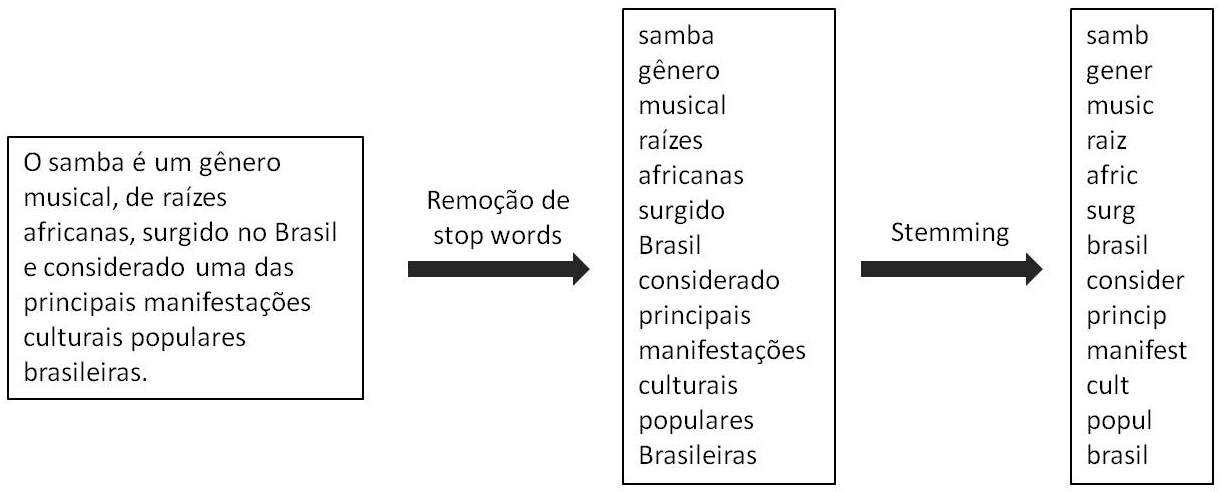
\includegraphics[width=0.45\textwidth]{exemplo-preprocessamento-noborder.jpg}
	\caption{Exemplo de pré-processamento.}
	\label{fig:exemplopreprocessamento}
  \end{figure}


Há ainda outros passos presentes nessa etapa como remoção de acentos, transformações de caixa, remoção de pontuação, os quais são relativamente simples e não requerem maiores detalhes.





%\subsection{Remoção de ruídos}

% Cabeçalhos e rodapés
As atas frequentemente contém trechos que podem ser considerados pouco informativos e descartados durante o pré-processamento, como cabeçalhos e rodapés que se misturam aos tópicos tratados na reunião, podendo ser  inseridos no meio de um tópico e criando uma quebra que prejudica tanto o algoritmo de segmentação, quanto a leitura do texto pelo usuário.
%%%%%%%%%%
% Numerais
%%%%%%%%%%
Também é comum o uso de numerais para marcação de páginas e linhas, da mesma forma, são pouco informativos e podem ser descartados.


%%%%%%%%%%
% Remoção de ruídos
%%%%%%%%%%
Nesse trabalho, esses elementos são removidos, uma vez que, o descarte não causa perca de informação e pode facilitar a identificação dos segmentos, pois melhora a coesão do texto. Outro benefício é manter o texto livre de trechos que fogem do assunto circundante.
%%%
% TODO: Como são removidos?
%%%


% por meio de heurísticas simples


%Como forma de padronização, as instituições acrescentam ao documento

%		passos menores
%		1 - heurística simples para remover cabeçalho e rodapé.
%		2 - remoção de numerais
%		3 - remoção de acentos, transformações de caixa, remoção de pontuação.
		
	% Esses passos são realizados internamente em cada algorímo, para que a saida seja legível ao usuário final.



\subsection{Identificação de candidatos}
	\label{subsec:indentificacaosentencas}
	
%%%%%%%%%%	
% Indicar unidade mínima de Segmento
%%%%%%%%%%
	
	
%	Como entrada para os 
%	Os algoritmos de segmentação devem ser
	É preciso fornecer aos algoritmos os candidatos iniciais a limites de segmento. Antes disso, é necessário escolher qual será a unidade de informação mínima que constitui um segmento. Baseando-se no estilo de escrita e considerando as pontuações dos textos, é possível indicar quebras de parágrafo, finais de sentenças ou mesmo palavras como elementos que encerram um segmento. 
	Ocorre que em atas de reunião é uma prática comum redigi-las de forma que o conteúdo discutido fica em parágrafo único, além disso, quebras de parágrafo são usados para formatação de outros elementos como espaço para assinaturas. 
	Indicar todo ponto entre \textit{token} como candidato obriga a ajustar posteriormente os segmentos de maneira a não quebrar uma ideia ou frase. Assim, neste trabalho, os finais de sentença são considerados unidades de informação e portanto, passíveis a limite entre segmentos. 
	
	Devido ao estilo de pontuação desses documentos, como encerrar sentenças usando um \textit{";"} e inserção de linhas extras, foram usadas as regras apresentadas no Algoritmo 1 para identificar os finais de sentenças.  


\begin{algorithm}
	\SetKwInOut{Input}{Entrada}
	\SetKwInOut{Output}{Saída}
	\SetKwBlock{Inicio}{início}{fim}
	\SetKwFor{ParaTodo}{para todo}{}{fim para todo}
	\SetKwIF{Se}{SenaoSe}{Senao}{}{}{senao se}{senao}{fim se}
	\SetKwFor{Para}{}{}{}

	
	\Input{Texto}
	\Output{Texto com identificações de finais de sentença}
	
	\ParaTodo {token, marcá-lo como final de sentença se:} {	

	Terminar com um \texttt{!}\\
	Terminar com um \texttt{.} e não for uma abreviação\\
	Terminar em \texttt{.?;} e:
		\Para{}{
			For seguido de uma quebra de parágrafo ou tabulação\\
			O próximo \textit{token} iniciar com  \texttt{(\{["'}\\
			O próximo \textit{token} iniciar com letra maiúscula\\
			O penúltimo caracter  for \texttt{)\}]"'}\\
		}
	}
	
	\caption{Identificação de finais de sentença}
\end{algorithm}






%A qualidade do algoritmo é sempre dependente da escrita correta! Ausência de emoticons, códigos de computador e gírias.





%Nas subseções a seguir serão expostas as alterações para aumentar a eficiência dos algoritmos e encontrar o melhor modelo para a tarefa de segmentar o texto das atas em tópicos.



%Tais aspectos não se aplicam ao contexto das atas, onde o estilo de escrita em forma de narrativa, prefere poupar o leitor de diálogos secundários durante transições de tópicos. 












